\documentclass[10pt,letter]{article}
\usepackage{amsmath}
\usepackage{amssymb}
\usepackage{graphicx}
\usepackage{bm}
\usepackage{amsthm}
\usepackage{array}
\usepackage[left=2.7cm,right=2.7cm,top=3cm,bottom=3cm]{geometry}
\usepackage{centernot}
%%\usepackage{stmaryrd}
\usepackage{hyperref}
\usepackage{multirow}
\usepackage{mathtools}
\usepackage{syntax}
\usepackage{mdframed}
\usepackage{dblfloatfix}
\usepackage{authblk}
\usepackage{rotating}
\mdfsetup{leftmargin=0cm,rightmargin=0cm,innertopmargin=0.5cm,innerbottommargin=0.5cm,linewidth=0.9}


\newtheorem*{note}{Note}
\theoremstyle{definition}
\newtheorem{problem}{Problem}
\newtheorem{lem}{Lemma}
\newtheorem*{theorem}{Theorem}
\newtheorem*{answer}{Answer}
\newtheorem*{ex}{Example}
\newtheorem*{base}{Base case}
\newtheorem*{inductive}{Inductive step}
\newtheorem*{cov}{Course-of-values inductive step}
\newtheorem*{conclusion}{Conclusion}
\setlength{\grammarparsep}{20pt} % increase separation between rules
\setlength{\grammarindent}{9em} % increase separation between LHS/RHS
\setlength{\columnsep}{2em}

\title{\bf Comparing and Integrating CVC4 and Alt-Ergo}
\author{Hanwen Wu}
\author{Wenxin Feng}
\affil{Department of Computer Science\\Boston University\\
\small\texttt{\{hwwu,wenxinf\}@bu.edu}}


\begin{document}
\maketitle

\begin{abstract}
This technical report summarizes the abilities of CVC4 and Alt-Ergo by testing them using SMT-LIB 2.0 benchmarks within the theories of boolean, free functions, integers, bit-vectors, and quantifiers. An extra $k$-induction benchmarks are also tested. The results show that CVC4 is both more powerful and more efficient than Alt-Ergo. They both can support quantifiers and non-linear integer arithmetic in a limited way. For induction over integers, they both can handle, and Alt-Ergo even outperform CVC4 for some inputs. We also implement a lightweight frontend calling both solvers to get the first valid response as the result.
\end{abstract}
\section{Overview}




Our main goal is thoroughly characterizing and comparing the abilities of two different SMT solvers, CVC4\cite{barrett:cvc4:2011} and Alt-Ergo\cite{alt-ergo} version 0.95.1. Since they both can take SMT-LIB 2.0\cite{bs2010} as their input language, we will also summarize it.

In this report, we will first of all, give a short introduction on SMT-LIB logic. Second, formally classifying input formulas using SMT-LIB logic. Third, introducing and summarizing the two solvers. Forth, carefully characterizing and comparing the abilities of the two solvers by testing them within different classes of formulas. And finally integrating them using a lightweight frontend written in C programming language.

\section{SMT-LIB 2.0 Logic}

In this section, we will briefly introduce SMT-LIB 2.0 logic so that we can more easily describe the classification of input formulas using SMT-LIB format later. It is developed as a standard logic to describe theories, input languages, and output languages. Currently it is supported by a variety of SMT solvers. They also hold competitions for SMT solvers every year, and have a collection of benchmarks which we will use for our tests.

\subsection{An Introduction}

Since we are going to use SMT-LIB 2.0 logic to describe the classification of formulas, it is necessary to understand the SMT-LIB 2.0 logic itself, which can be used as an input language for both solvers (Alt-Ergo, CVC4).

SMT-LIB 2.0 is basically a version of many-sorted first-order logic with equality\cite{bs2010}. It provides us the ability to write formulas, define theories and logics, and interact with provers using scripts. Provers that support SMT-LIB 2.0 should implement required functionalities and use correct semantics.

\subsubsection{Sets of Symbols}

These are part of the sets defined by SMT-LIB 2.0\cite{barrett:smt-lib:2010}. They are alphabets of the logic, namely, the sources of symbols. These symbols will be used in the following subsections.
\begin{itemize}
\item $\mathcal{S}$: Infinite set of sort symbols, containing $\tt bool$.
\item $\mathcal{U}$: Infinite set of sort parameters.
\item $\mathcal{X}$: Infinite set of variables.
\item $\mathcal{F}$: Infinite set of function symbols.
\item $\mathcal{B}$: Boolean values \{{\bf true, false}\}.
\item \qquad$\vdots$
\end{itemize}



\subsubsection{Sorts}

SMT-LIB 2.0 is a sorted logic. Sorts over a set of sort symbols $\mathcal{S}$ are defined as Sort($\mathcal{S}$). Sorts are defined inductively as follows.

\begin{itemize}
\item $\sigma \in \mathcal{S}$ of arity 0 is a sort.
\item $\sigma,\sigma_1, \sigma_2, \sigma_3, \ldots, \sigma_n$ is a sort if $\sigma \in \mathcal{S}$ is of arity $n$, and $\sigma_1$ to $\sigma_n$ are sorts.
\end{itemize}
The second item uses sorts to form new sorts. A list of integers can be a good example.

\subsubsection{Signature}

Basically, a signature $\Sigma$ defines sort symbols and arities, function symbols and ranks, some variables and their sorts.

\begin{itemize}
\item $\Sigma^\mathcal{S} \subset \mathcal{S}$: sort symbols, containing $\tt bool$.
\item $\Sigma^\mathcal{F} \subset \mathcal{F}$: function symbols, containing equality, conjunction, and negation.
\item $\Sigma^\mathcal{S}$ to $\mathbb{N}$: a total mapping from sort symbol to its arity, including $\tt bool \Rightarrow 0$.
\item $\Sigma^\mathcal{F}$ to Sort($\Sigma^\mathcal{S}$)$+$: a left total mapping from a function symbol to its rank, containing $=(\sigma, \sigma, {\tt bool} )$, $\neg({\tt bool},{\tt bool})$, $\wedge ({\tt bool}, {\tt bool}, {\tt bool})$.
\item $\mathcal{X}$ to Sort($\Sigma^\mathcal{S}$): a partial mapping from a variable to its sort.
\end{itemize}

In the logic definitions of SMT-LIB, we will see ``expended signature'' a lot. We will formalize the expansion methods in later sections.

\subsubsection{Formulas}

In SMT-LIB 2.0, formulas are well sorted terms of sort $\tt bool$ over $\Sigma$. In actual scripts, all the formulas are being treated as closed formulas. This is possible since non-closed formulas can be quantified using existential quantifier, as far as its satisfiability is concerned.

\subsubsection{Structure}

A structure $\bf A$ in SMT-LIB 2.0 can be regarded as a model. It is defined as a tuple. \[\bf{A}\it = \{A,\sigma^{\bf A}\footnote{$\sigma^{\bf A}$ is called the extension of $\sigma$ in $\bf A$.}\ ,(f:\sigma)^{\bf A},(f:\sigma_1,\sigma_2,\ldots,\sigma_n,\sigma)^{\bf A} \}\]
And the meaning of these four elements are the followings.
\begin{itemize}
\item $A$: the universe (of values) of $\bf A$, including $\tt bool^{\bf A} = $ \{{\bf true, false}\}.
\item $\sigma^{\bf A} \subset A$: gives the sort $\sigma \in $ Sort($\Sigma^\mathcal{S}$) a universe $\sigma^{\bf A} \subset A$. For example, $\tt bool^{\bf A}$ is \{{\bf true, false}\} $ \subset \it A$. $\tt int^{\bf A}$ could be all the integers $\mathbb{Z} \subset A$.
\item $(f:\sigma)^{\bf A} \in \sigma^{\bf A}$: gives the constant symbol $f:\sigma$ a value in the universe of $\sigma$
\item $(f:\sigma_1,\sigma_2,\ldots,\sigma_n,\sigma)^{\bf A}$: defines the function symbol as a relation from $(\sigma_1,\sigma_2,...,\sigma_n)^{\bf A}$ to $\sigma^{\bf A}$. This must include the equality relations (or identity predicate over $\sigma^{\bf A}$, that is $\tt = (\sigma, \sigma, bool)$ as standard equality relations from $(\sigma^{\bf A}, \sigma^{\bf A})$ to \{{\bf true, false}\}).
\end{itemize}

\subsubsection{Valuation and Interpretation}

Valuation $v$ is a partial mapping from $\mathcal{X} \times$Sort($\Sigma^\mathcal{S}$) to $\sigma^{\bf A}$. That is to give variable $x$ of sort $\sigma$ a value in $\sigma^{\bf A}$.

Interpretation $\mathcal{I}$ is defined as $\mathcal{I} = ({\bf A}, v)$, that is the structure together with the valuation make the $\Sigma$-interpretation.

$\mathcal{I}$ will assign meanings to well-sorted terms by uniquely mapping them into the $\bf A$. And that is the semantic.

As long as we have semantics, we can talk about satisfiability. If $\varphi$ is mapped to {\bf true} by some $\mathcal{I}$, then it is satisfiable. If $\varphi$ is not closed, we say $\mathcal{I} = ({\bf A}, v)$ makes true $\varphi$. If $\varphi$ is closed, we say the structure $\bf A$ makes true $\varphi$. (Since it doesn't matter what valuation it is), and that means $\bf A$ is a model of $\varphi$.

\subsubsection{Theories}
Theory is a very important concept here. SMT stands for Satisfiability Modulo Theory, that is to check the satisfiability of a given logical formula within some background theories. Traditionally, a theory is a set of enough axioms, with which we can induct the formula. But here a theory $\mathcal{T}$ consists of three parts.
\begin{itemize}
\item Signature: $\Sigma$
\item Models: A set of $\Sigma$-structures, all of which are models of the theory.
\item Axioms: This is actually part of the models, and is left for the people who implement solvers. Take integer theory as an example. Since we have the plus sign in our signature (we just denote it as $\tt ADD$, so that we know it is only a symbol, not the actual operation), we will have an axiom like $\forall x:{\tt int}.\forall y:{\tt int}. \exists z:{\tt int}. {\tt ADD}(x,y,z) \leftrightarrow x + y = z$. Therefore, our model (or structure) must contain the correct relations to map $\tt ADD$ to the actual addition operation to satisfy this axiom. Also, some theories, like real numbers, include those axioms as plain text, like associativity, commutativity, etc.

\end{itemize}

The SMT-LIB 2.0 standard has defined six theories. They are Core (for propositional logic), Integer, Real, Real and Integer, Fixed Size Bit-Vector, and Arrays. Each of them defines corresponding signature, and models. The actual implementations are left for the provers.

\subsubsection{Logics}
Logic in SMT-LIB is also very important. It is a sublogic of SMT-LIB logic with restrictions, and is based on some theories. Common restrictions are
\begin{itemize}
\item fixing a signature $\Sigma$ and its theory $\mathcal{T}$
\item restricting structures to the models of $\mathcal{T}$
\item restricting input sentences as subset of $\Sigma$-sentences
\end{itemize}

The SMT-LIB standard has classify formulas into many well-defined logics, including QF-UF, QF-LIA, QF-NIA, QF-IDL, QF-LRA, QF-NRA, QF-RDL, QF-BV, QF-AX, etc. We will not discuss them all, but focusing on integers and fixed-size bit-vectors.

\subsection{Theory}
In the following, we are going to present some abstract definition of different theories in SMT-LIB 2.0. Note that the Core theory is included in all other theories by default.

In all the figures, function symbols will only be applied to well-sorted terms according to their own function ranks/signatures/definitions.


\subsubsection{Core Theory}
Core Theory is all about boolean sort and boolean functions/constants. It is the very base for all other theories.

Beyond propositional logic, there are two more features in the Core theory. The first is equality/distinction. These two function symbols are defined not only for $\tt bool$, but also for all potential sorts in an expanded signature. The second is $\bf ite$, which is the $\bf if-then-else$ operator. It is also defined for other sorts.


\begin{table*}[!h]
\begin{mdframed}
\centering
\begin{tabular}{r c l}
sort\qquad $\alpha$ & $\Coloneqq$ & \tt bool\\
\\
function\qquad $f$ & $\Coloneqq$ & \bf true \rm : \tt bool $\mid$ \bf false \rm : \tt bool \\
& $\mid$ & (\bf not \tt\ bool\rm) : \tt bool $\mid$ \rm(\bf and \tt\ bool bool\rm) : \tt bool \\
& $\mid$ & (\bf or \tt\ bool bool\rm) : \tt bool \\
& $\mid$ & (\bf xor \tt\ bool bool\rm) : \tt bool \\
& $\mid$ & ($\Rightarrow$ \tt\ bool bool\rm) : \tt bool $\mid$ \rm($=$ \tt\ $\alpha$ $\alpha$\rm) : \tt bool\\
& $\mid$ & (\bf distinct \tt\ $\alpha$ $\alpha$\rm) : \tt bool $\mid$ \rm(\bf ite \tt\ bool $\alpha$ $\alpha$\rm) : $\alpha$\\
\\
term\qquad $t$ & $\Coloneqq$ & \bf true $\mid$ false\\
& $\mid$ & (\bf not \rm $t$) $\mid$ (\bf and \rm $t$ $t$) $\mid$ (\bf or \rm $t$ $t$) $\mid$ (\bf xor \rm $t$ $t$) \\
& $\mid$ & ($\Rightarrow$ $t$ $t$) $\mid$ ($=$ $t$ $t$) $\mid$ (\bf distinct \rm $t$ $t$) $\mid$ (\bf ite \rm $t$ $t$ $t$)
\end{tabular}
\end{mdframed}
\caption{Core Theory}
\end{table*}


\subsubsection{Integer Theory}
Integer Theory defines the integer domain, and operations over integers. It is a superset of Core theory, thus includes all the sorts and function symbols defined in Core theory.

Note that the Integer theory itself doesn't have any restriction on linear or nonlinear operations. They should instead be defined in logics based on Integer theory. Also, the division, modulo operations here are defined for integers which actually involve flooring and ceiling.

\begin{table*}[!h]
\begin{mdframed}
\centering
\begin{tabular}{r c l}
sort\qquad $\alpha$ & $\Coloneqq$ & \tt bool $\mid$ \tt int\\
\\
function\qquad $f$ & $\Coloneqq$ & $\ldots$ \\
& $\mid$ & $\mathbb{Z}$ \rm : \tt int\\
& $\mid$ & ($-$ \tt\ int\rm) : \tt int $\mid$ \rm($-$ \tt\ int int\rm) : \tt int\\
& $\mid$ & ($+$ \tt\ int int\rm) : \tt int $\mid$ \rm($\times$ \tt\ int int\rm) : \tt int\\
& $\mid$ & (\bf div \tt\ int int\rm) : \tt int $\mid$ \rm(\bf mod \tt\ int int\rm) : \tt int\\
& $\mid$ & (\bf abs \tt\ int\rm) : \tt int \\
& $\mid$ & ($\leqslant$ \tt\ int int\rm) : \tt bool $\mid$ \rm($<$ \tt\ int int\rm) : \tt bool\\
& $\mid$ & ($\geqslant$ \tt\ int int\rm) : \tt bool $\mid$ \rm($>$ \tt\ int int\rm) : \tt bool\\
& $\mid$ & ( (_\ \bf\ divisible \rm\ $n$) \tt\ int\rm) : \tt bool \rm\qquad($n$ is a positive integer)\\
\\
term\qquad $t$ & $\Coloneqq$ & $\ldots$ \\
& $\mid$ & $\ldots\quad-1,0,1\quad\ldots$\\
& $\mid$ & ($-$ $t$) $\mid$ ($-$ $t$ $t$) $\mid$ ($+$ $t$ $t$) $\mid$ ($\times$ $t$ $t$) \\
& $\mid$ & (\bf div \rm $t$ $t$) $\mid$ (\bf mod \rm $t$ $t$) $\mid$ (\bf abs \rm $t$)\\
& $\mid$ & ($\leqslant$ $t$ $t$) $\mid$ ($<$ $t$ $t$) $\mid$ ($\geqslant$ $t$ $t$) $\mid$ ($>$ $t$ $t$)\\
& $\mid$ & ( (_\ \bf\ divisible \rm\ $n$\ )\ $t$\ )
\end{tabular}
\end{mdframed}
\caption{Integer Theory}
\end{table*}


\subsubsection{Fixed-Size Bit-Vectors Theory}
This theory defines a series of sorts for different size of bit-vectors. Concatenation and extraction of bit-vectors, and the usual logical and arithmetic operations are also defined. The universe of bit-vectors theory is those numeral constants in bit-vector format. They are defined using a SMT-LIB syntax of the form {\tt \#b}X and {\tt \#x}X for binary and hexadecimal constants.

In the table, we use {\tt bv} for ({\tt \_\ BitVec $m$}), and omitting the size of the bit-vectors, only for layout reasons.


\begin{table*}[!h]
\begin{mdframed}
\centering
\begin{tabular}{r c l}
sort\qquad $\alpha$ & $\Coloneqq$ & \tt bool \\
& $\mid$ & \rm(\tt \_\ BitVec $m$\rm)\it\quad \rm($m$ \rm is a positive integer, we use {\tt bv} for short)\\
\\
function\qquad $f$ & $\Coloneqq$ & $\ldots$ \\
& $\mid$ & {\tt \#b}X \rm : \tt bv \rm\qquad (all binary constants)\\
& $\mid$ & {\tt \#x}X \rm : \tt bv \rm\qquad (all hexadecimal constants)\\
& $\mid$ & (\bf concat \tt\ bv bv\rm) : \tt bv \\
& $\mid$ & \rm(\ (\_\tt\ {\bf extract}\ $i$\ $j$\rm) \tt\ bv\rm) : \tt bv\rm\qquad ($i, j$ specify the range)\\
& $\mid$ & (\bf bvnot \tt\ bv\rm) : \tt bv \rm$\mid$ (\bf bvneg \tt\ bv\rm) : \tt bv \\
& $\mid$ & (\bf bvand \tt\ bv bv\rm) : \tt bv \rm$\mid$ (\bf bvor \tt\ bv bv\rm) : \tt bv \\
& $\mid$ & (\bf bvadd \tt\ bv bv\rm) : \tt bv \rm$\mid$ (\bf bvmul \tt\ bv bv\rm) : \tt bv \\
& $\mid$ & (\bf bvudiv \tt\ bv bv\rm) : \tt bv \rm$\mid$ (\bf bvurem \tt\ bv bv\rm) : \tt bv \\
& $\mid$ & (\bf bvshl \tt\ bv bv\rm) : \tt bv \rm$\mid$ (\bf bvlshr \tt\ bv bv\rm) : \tt bv \\
& $\mid$ & (\bf bvult \tt\ bv bv\rm) : \tt bool \\
\\
term\qquad $t$ & $\Coloneqq$ & $\ldots$ \\
& $\mid$ & {\tt \#b}X \rm\qquad (all binary constants)\\
& $\mid$ & {\tt \#x}X \rm\qquad (all hexadecimal constants)\\
& $\mid$ & (\bf concat \rm $t$ $t$) $\mid$ (\ (\_\tt\ {\bf extract} \rm $i$ $j$)\ $t$)\\
& $\mid$ & (\bf bvnot \rm $t$) $\mid$ (\bf bvneg \rm $t$) $\mid$ (\bf bvand \rm $t$ $t$) $\mid$ (\bf bvor \rm $t$ $t$)\\
& $\mid$ & (\bf bvadd \rm $t$ $t$) $\mid$ (\bf bvmul \rm $t$ $t$) $\mid$ (\bf bvudiv \rm $t$ $t$) $\mid$ (\bf bvurem \rm $t$ $t$)\\
& $\mid$ & (\bf bvshl \rm $t$ $t$) $\mid$ (\bf bvlshr \rm $t$ $t$) $\mid$ (\bf bvult \rm $t$ $t$) \\
\end{tabular}
\end{mdframed}
\caption{Fixed-Size Bit-Vectors Theory}
\end{table*}


\subsection{Logic}

Logic is the main tool we use for classifying formulas and testing solver abilities. In the followings, we will formalize the definition of various logics of SMT-LIB.

\subsubsection{Quantifier-Free Uninterpreted Functions}
Closed quantifier-free formulas built over an arbitrary expansion of the Core signature with free sort and function symbols \cite{bs2010}. Users can define their own sorts and function symbols, but all of them are abstract. Functions can contain variables, but they must be bounded by \bf let \rm binder, so that the formulas are closed.

\begin{table*}[!h]
\begin{mdframed}
\centering
\begin{tabular}{r c l}
sort\qquad $\alpha$ & $\Coloneqq$ & $\ldots$ $\mid$ $\alpha'$ ($\alpha^*$)\rm\qquad(user defined, abstract)\\
\\
function\qquad $f$ & $\Coloneqq$ & $\ldots$ $\mid$ \rm ($f'$ $\alpha^*$) : $\alpha$\qquad(user defined, abstract)\\
\\
term\qquad $t$ & $\Coloneqq$ & $\ldots$ \\
& $\mid$ & (\bf\ let \rm ( bindings$^+$ ) $t$\ )\\
& $\mid$ & ($f$ $t^*$)
\end{tabular}
\end{mdframed}
\caption{QF-UF Logic}
\end{table*}

\subsubsection{Quantifier-Free Linear Integer Arithmetic}
Closed quantifier-free formulas built over an arbitrary expansion of the
Integer Theory with free {\it constant} symbols, but whose terms of sort {\tt int}
are all linear \cite{bs2010}. Note that user can only define constants, not arbitrary functions who take one or more arguments. User can't define sort either. Also, non-linear functions like \bf div\rm, \bf mod\rm, \bf abs \rm and non-linear $\times$ are not allowed.

\begin{table*}[!h]
\begin{mdframed}
\centering
\begin{tabular}{r c l}
sort\qquad $\alpha$ & $\Coloneqq$ & \tt bool $\mid$ int\\
\\
function\qquad $f$ & $\Coloneqq$ & $\ldots$ $\mid$ \rm $f'$ : $\alpha$\qquad(user defined constant)\\
\\
term\qquad $t$ & $\Coloneqq$ & $\ldots$ \\
& $\mid$ & $\ldots\quad-1,0,1\quad\ldots$\\
& $\mid$ & ($-$ $t$) $\mid$ ($-$ $t$ $t$) $\mid$ ($+$ $t$ $t$) \\
& $\mid$ & ($\times$ $c$ $t$) $\mid$ ($\times$ $t$ $c$) \qquad($c$ is an integer literal)\\
& $\mid$ & ($\leqslant$ $t$ $t$) $\mid$ ($<$ $t$ $t$) $\mid$ ($\geqslant$ $t$ $t$) $\mid$ ($>$ $t$ $t$)\\
& $\mid$ & ( (_\ \bf\ divisible \rm\ $n$ )\ $t$\ )\\
& $\mid$ & (\bf\ let \rm ( bindings$^+$ ) $t$\ )\\

\end{tabular}
\end{mdframed}
\caption{QF-LIA Logic}
\end{table*}

\section{Comparing CVC4 and Alt-Ergo}

In this section, we will give a short summary of both solvers first. Their overall architectures, built-in theories, combination methods, and unique features will be briefly discussed. Then we will summarize our test methods and results to show their capabilities within different sub logics using SMT-LIB 2.0 benchmarks.

\subsection{CVC4}

CVC4, the fifth generation of Cooperating Validity Checker from NYU and U Iowa, is a DPLL({\it T}) solver with a SAT solver core and a delegation path to different decision procedure implementations, each in charge of solving formulas in some background theory\cite{barrett:cvc4:2011}. It works for first-order logics. It has implemented decision procedures for the theory of uninterpreted/free functions, arithmetic(integer, real, linear, non-linear), arrays, bit-vectors and datatypes. It uses a combination method based on Nelson-Oppen to cooperate different theories. Also, it supports quantifiers through heuristic instantiaion\footnote{See \url{http://cvc4.cs.nyu.edu/wiki/About_CVC4}} and has the ability to generate model. By our tests of $k$-induction over linear integer arithmetic, it supports induction very well.

For both satisfiable/unsatisfiable formulas, CVC4 will come up with the correct answer

\subsection{Alt-Ergo}

Alt-Ergo is dedicated to program verification. It works in first-order logic. It uses a CC(X)\footnote{CC(X): Congruence closure modulo X}, a variant of Shostak algorithm, to combine free theory with equality and an arbitrary solvable built-in theory X\cite{conchonHDR2012}. Alt-Ergo has implemented decision procedures for the theory of uninterpreted/free functions, arithmetic(integer, real, linear, non-linear), arrays, bit-vectors, datatypes, etc. It also has direct support for polymorphism in its native input language. Associative and commutative symbols are being handled specially using its AC(X) theory to boost the performance. It has some support for universal and existential quantifiers through instantiation. It has the ability to generate proof. Also, by our test of $k$-induction, it can prove them quickly.

Alt-Ergo can handle {\tt unsat} formulas correctly, but only returns {\tt unknown} for {\tt sat} formulas.

Since integer theory are intensively used in program verification, Alt-Ergo actually put its efforts in the combination of empty/free theory with integer arithmetic theory. Alt-Ergo uses a Simplex-based extension of Fourier-Motzkin for solving linear integer arithmetic\cite{bobot:hal-00687640}.

\subsection{Testing Both Solvers}

\subsubsection{Benchmarks}

SMT-LIB community has been contributing benchmarks and holding competitions for several years\cite{bs2010}. It can be considered as a good standard benchmark for SMT solvers. We have select integers, bit-vectors, and quantifiers related benchmarks for our test. They are QF-IDL, QF-NIA, QF-UFBV, QF-UFLIA, UFNIA, QF-BV, QF-LIA, QF-UF, QF-UFIDL.

We also select the Bounded Model Checking and $k$-induction problems within QF-LIA benchmarks from 2012 SMT Competition\footnote{\url{http://smtcomp.sourceforge.net/2012/application.shtml}}\cite{cok20122012} 
to test their abilities of proving inductive facts.

All of the benchmarks are in the SMT-LIB 2.0 format, most of which should be handled by both solvers. But in practice, Alt-Ergo reports typing error and parsing error on some test inputs because its currect version 0.95.1 doesn't fully support it yet. And also, some of the benchmarks don't indicate expected results. They are either {\tt unknown} or not available at all. Therefore, we will only consider those can be handled by both solvers, and have an expected answer of {\tt sat/unsat} as valid benchmarks when we analysis the result.

\subsubsection{Testing Methods}

We have wrote a testing script to run the test. Basicly, it will first randomly select test inputs from all the benchmarks. Second, both solvers will be invoked for each input, individually, not simultaneously. Third, their execution time will be captured by Unix {\tt time} utility, and the real wall time will be considered as their execution time. Forth, there is a timeout of 30 seconds. If any of them reach 30 seconds, it will be killed. Fifth, since Alt-Ergo can't handle inputs with an expected answer of {\tt sat}, we will just skip that for Alt-Ergo, and only use that input as a measure of efficiency/capability for CVC4 only.

For BMC and $k$-induction problems, we have a different strategy. Each of those tests consists of multiple checking points, which require the solver to solve them incrementally. Therefore we setup a timeout of 15 seconds, to compare how much problems they can solve in a limited time.

We run the tests on a Core i5-3320M 2.6GHz dual core CPU with 8GB memory, on Ubuntu 13.04 32bit operating system. During testing, no other job is allowed.



\subsection{Testing Results}

\subsubsection{General}

The general test results are shown in Table \ref{t:result} and Figure \ref{f:unsatcap} for {\tt unsat} tests for both solvers, and Figure \ref{f:satcap} for {\tt sat} tests for CVC4 only. The timeout rate is relatively high in some divisions, due to the small 30 seconds timeout. And this is partly because we don't have enough time and computation resources to perform long enough tests. The error rate is also relatively high. For Alt-Ergo, this is mainly because it doesn't fully support SMT-LIB 2.0 standard, and particularly, its bit-vectors and typing parts. Alt-Ergo supports its native input language very well, but there seems not to be a good translation from SMT-LIB format into its native format. For CVC4, the error mostly comes from big input formulas, which cause CVC4 to throw some unexpected exceptions.

For those parts which they both can handle, namely QF-IDL, QF-UFLIA, QF-UF and UFNIA, they will generally respond quickly. For solver ability, CVC4 always wins with very high solved percentage. For solver efficiency, CVC4 also beats Alt-Ergo.

For the following sections, we will first compare them for those {\tt unsat} inputs. And at the last, we will talk about {\tt unsat} formulas for CVC4 only, and then BMC and $k$-induction problems.

\begin{table*}[!ht]
\small
\centering
\begin{tabular}{|cc|c|cccc|}
\hline
 \bf Logic & \bf Total &\bf Solver &\bf Correct &\bf Timeout &\bf Exception & \bf Unknown\\\hline
  \multirow{2}{*}{QF-BV} & \multirow{2}{*}{16} & Alt-Ergo & 0 & 0 & 100\% & 0\\
  & & CVC4 & 81.25\% & 12.50\% & 6.25\% & 0\\\hline
  \multirow{2}{*}{QF-IDL} & \multirow{2}{*}{106} & Alt-Ergo & 10.38\% & 67.92\% & 13.21\% & 8.49\%\\
  &  & CVC4 & 63.21\% & 36.79\% & 0 & 0\\\hline
  \multirow{2}{*}{QF-LIA} & \multirow{2}{*}{143} & Alt-Ergo & 0 & 100\% & 0 & 0\\
  &  & CVC4 & 95.80\% & 4.20\% & 0 & 0\\\hline
  \multirow{2}{*}{QF-NIA} & \multirow{2}{*}{58} & Alt-Ergo & 0 & 0 & 96.55\% & 3.45\%\\
  &  & CVC4 & 60.34\% & 0 & 29.31\% & 10.34\%\\\hline
  \multirow{2}{*}{QF-UF} & \multirow{2}{*}{195} & Alt-Ergo & 36.41\% & 63.08\% & 0.51\% & 0\\
  &  & CVC4 & 97.95\% & 2.05\% & 0 & 0\\\hline
  \multirow{2}{*}{QF-UFBV} & \multirow{2}{*}{31} & Alt-Ergo & 0 & 0 & 100\% & 0\\
  &  & CVC4 & 19.35\% & 80.65\% & 0 & 0\\\hline
  \multirow{2}{*}{QF-UFIDL} & \multirow{2}{*}{91} & Alt-Ergo & 0 & 1.10\% & 98.90\% & 0\\
  &  & CVC4 & 57.14\% & 42.86\% & 0 & 0\\\hline
  \multirow{2}{*}{QF-UFLIA} & \multirow{2}{*}{163} & Alt-Ergo & 6.75\% & 6.75\% & 86.50\% & 0\\
  &  & CVC4 & 95.71\% & 4.29\% & 0 & 0\\\hline
  \multirow{2}{*}{UFNIA} & \multirow{2}{*}{1562} & Alt-Ergo & 9.80\% & 29.64\% & 60.37\% & 0.19\%\\
  &  & CVC4 & 40.59\% & 31.82\% & 27.59\% & 0\\\hline
\end{tabular}
\caption{Capabilities of CVC4 and Alt-Ergo for {\tt unsat} Tests}
\label{t:result}
\end{table*}

\begin{table*}[!ht]
\small
\centering
\begin{tabular}{|cc|c|cc|}
\hline
\bf  Logic & \bf Total &\bf Solver & \bf Correct & \bf Avg.Time \tiny{(sec)}\\\hline
  \multirow{2}{*}{QF-BV} &\multirow{2}{*}{16} & Alt-Ergo & 0 &  \\
  && CVC4 & 13 & 16.31 \\\hline
  \multirow{2}{*}{QF-IDL} &\multirow{2}{*}{106} & Alt-Ergo & 11 & 2.56\\
  &&  CVC4 & 67 & 2.80 \\\hline
  \multirow{2}{*}{QF-LIA} &\multirow{2}{*}{143} & Alt-Ergo & 0 & \\
  && CVC4 & 137 & 4.05\\\hline
  \multirow{2}{*}{QF-NIA} &\multirow{2}{*}{58} &  Alt-Ergo & 0 & \\
  & &  CVC4 & 35 & 0.10\\\hline
  \multirow{2}{*}{QF-UF} & \multirow{2}{*}{195} & Alt-Ergo & 71 & 9.51\\
  &  & CVC4 &191 & 1.04\\\hline
  \multirow{2}{*}{QF-UFBV} &  \multirow{2}{*}{31} &  Alt-Ergo & 0 & \\
  &  & CVC4 & 6 & 4.02\\\hline
  \multirow{2}{*}{QF-UFIDL} & \multirow{2}{*}{91} & Alt-Ergo & 0 & \\
  &  & CVC4 & 52 & 3.43\\\hline
  \multirow{2}{*}{QF-UFLIA} & \multirow{2}{*}{163} & Alt-Ergo & 11 & 5.07\\
  &  & CVC4 & 156 & 0.70\\\hline
  \multirow{2}{*}{UFNIA} & \multirow{2}{*}{1562} &Alt-Ergo & 153 & 3.08\\
  &  & CVC4 & 634 & 2.57\\\hline
\end{tabular}
\caption{Efficiencies of CVC4 and Alt-Ergo for {\tt unsat} Tests}
\label{t:eff}
\end{table*}


\begin{sidewaysfigure}[!h]
\centering
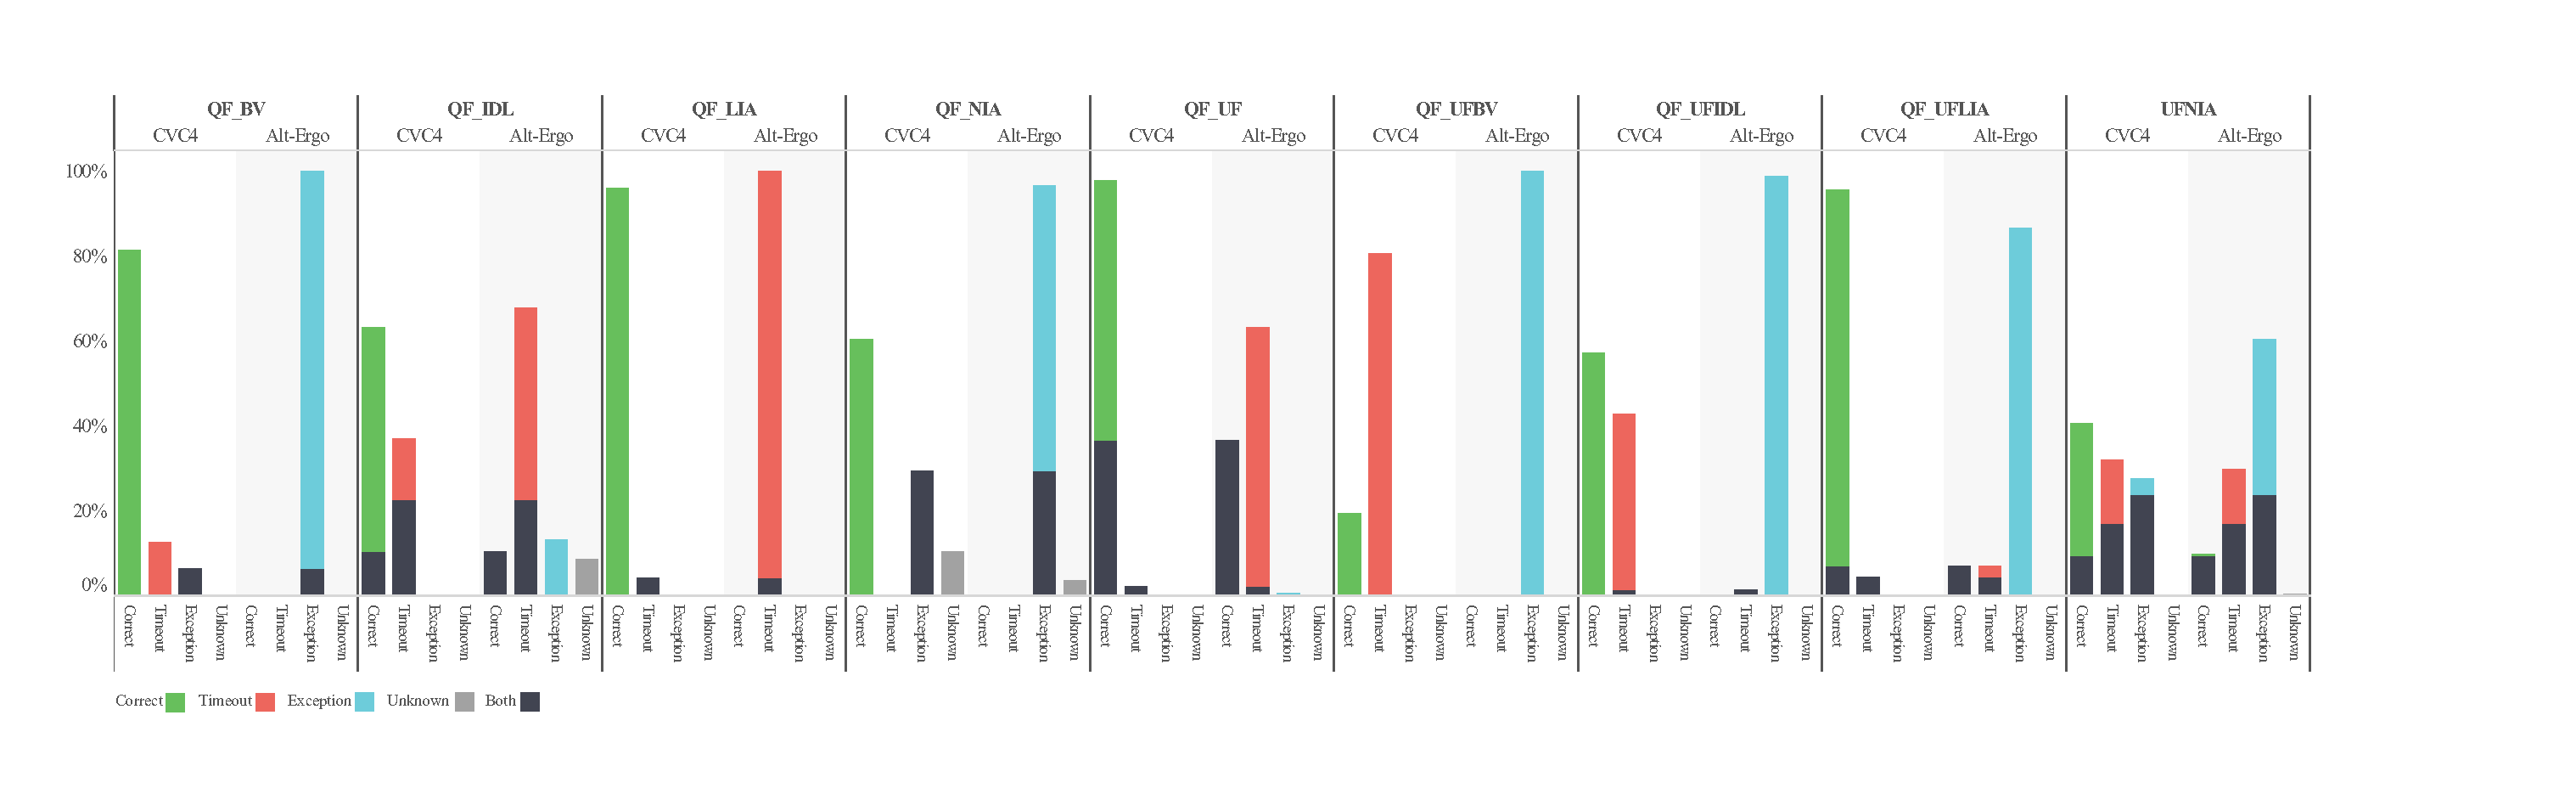
\includegraphics[scale=0.45]{./testanalysis/unsatcap.pdf}
\caption{Capabilities of CVC4 and Alt-Ergo on {\tt unsat} Tests}
\label{f:unsatcap}
\end{sidewaysfigure}


\begin{sidewaysfigure}[!h]
\centering
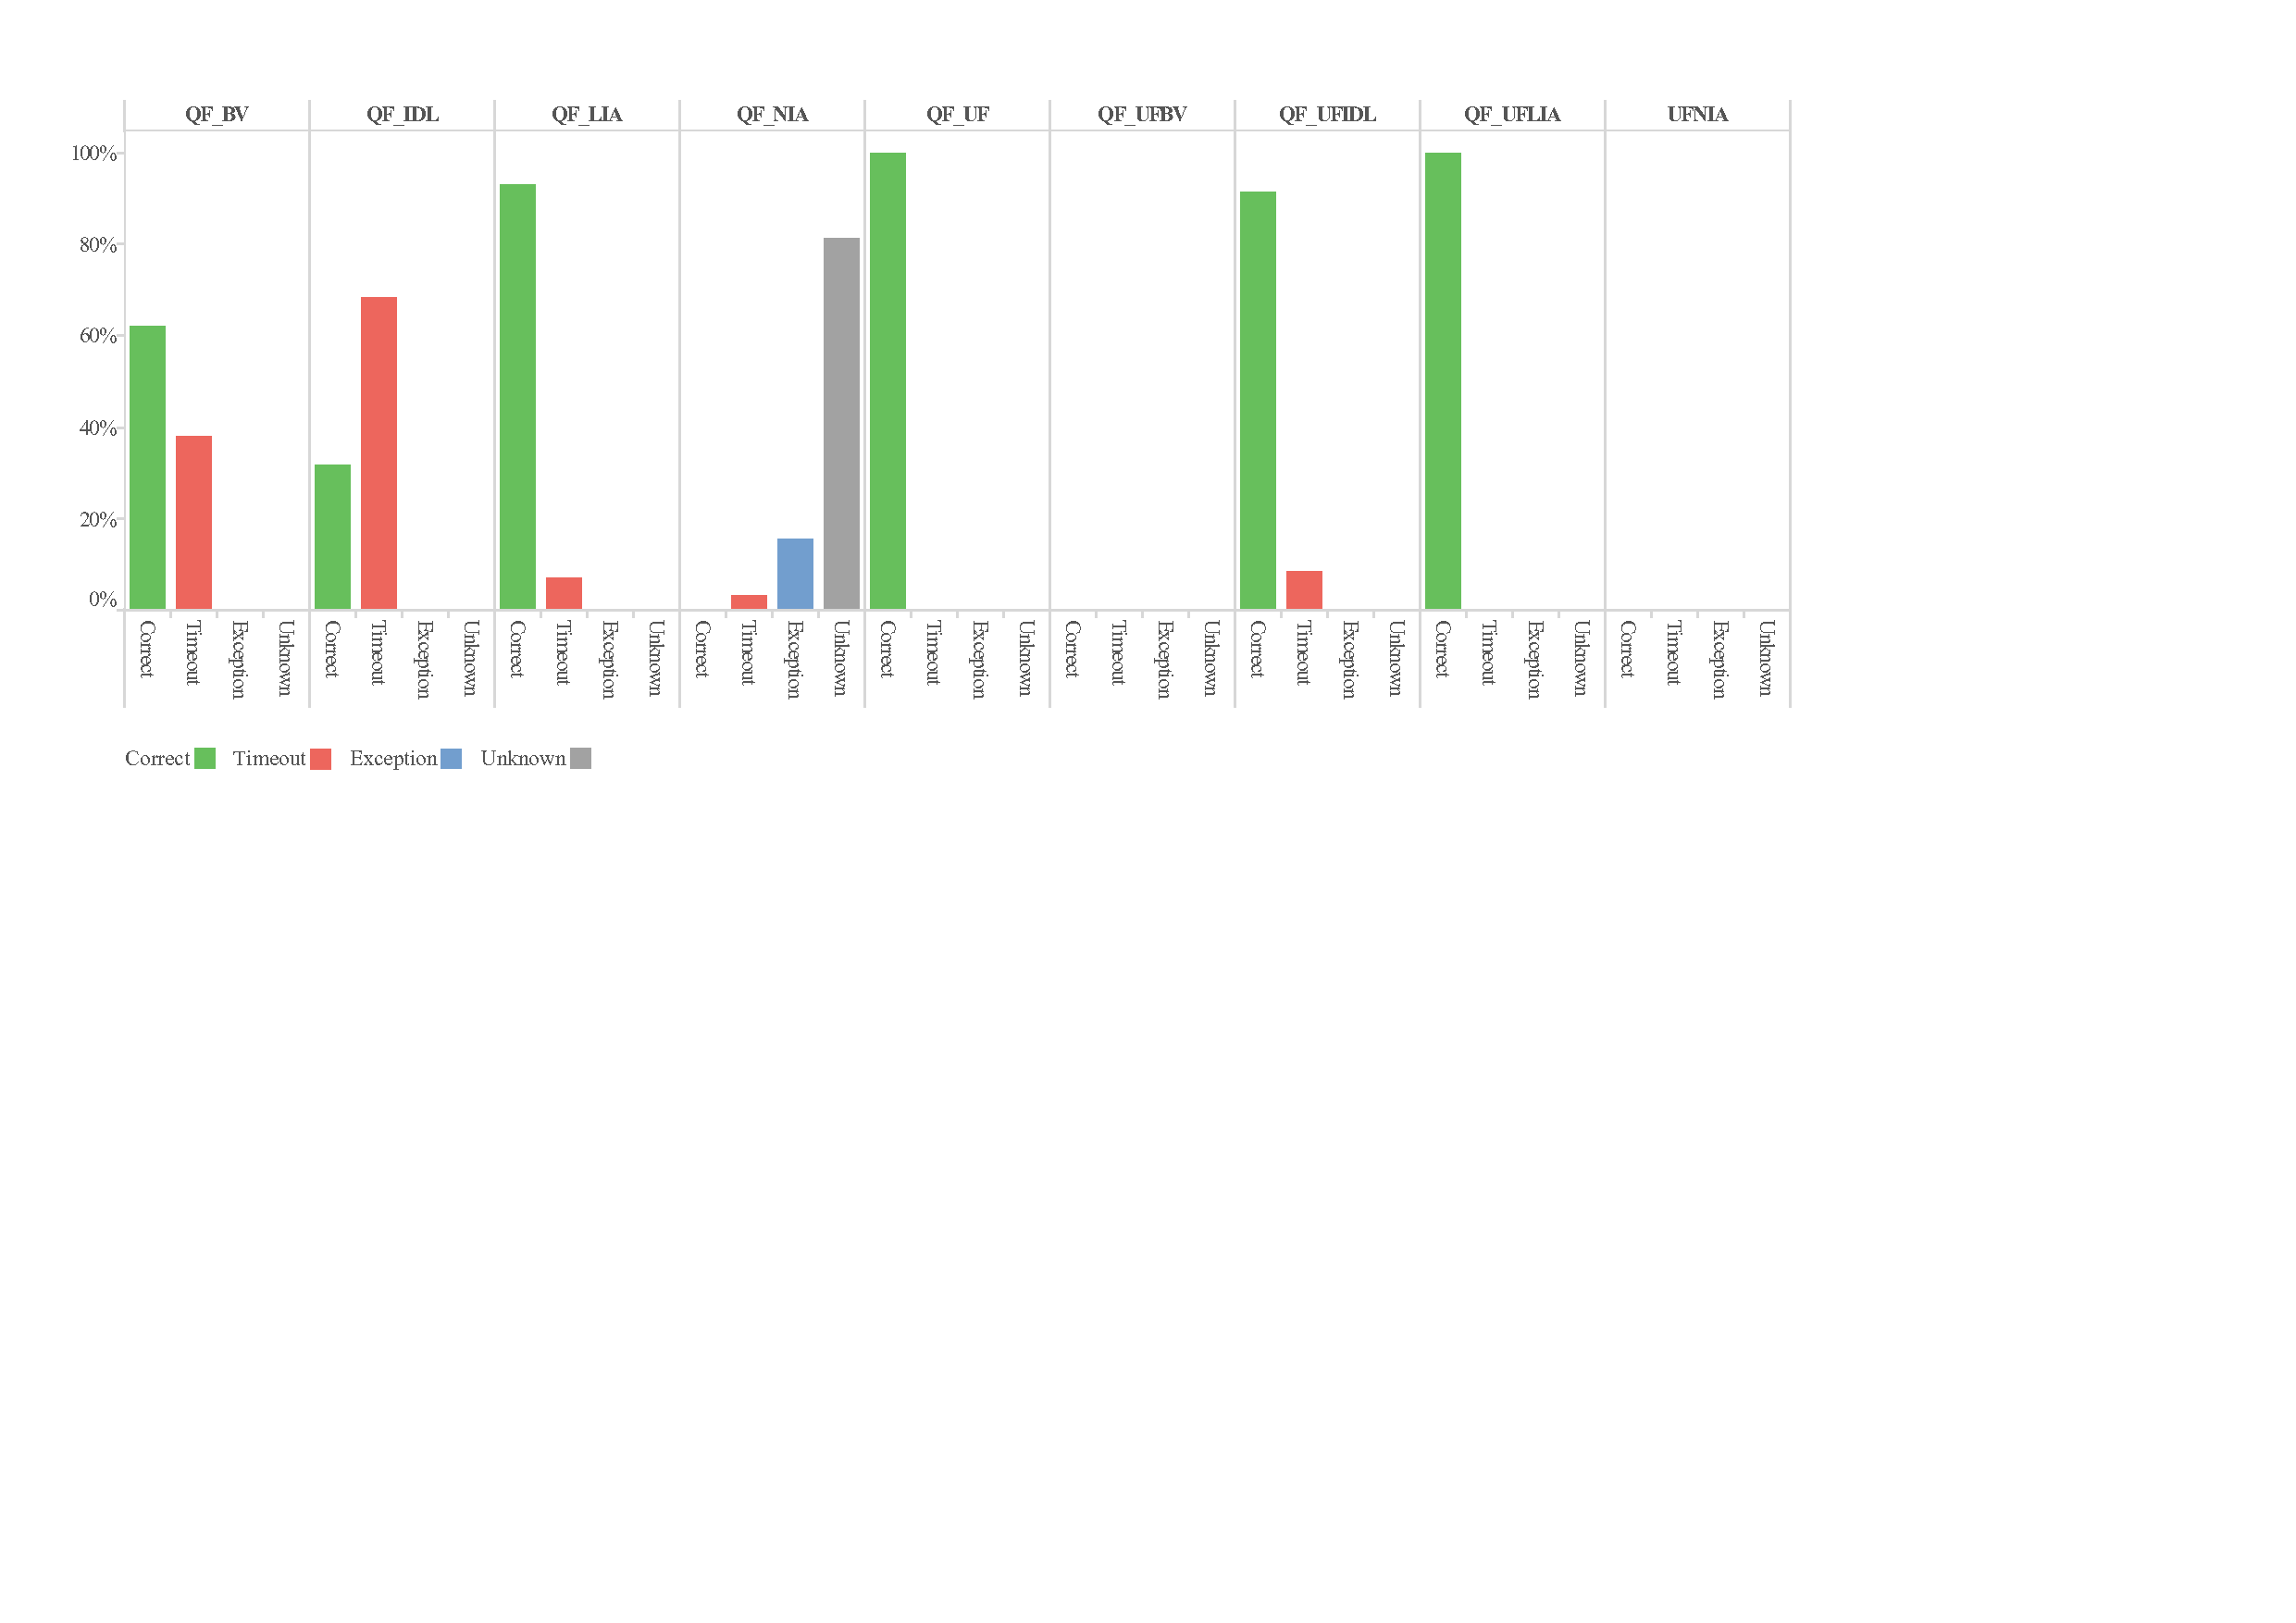
\includegraphics[scale=0.45]{./testanalysis/satcap.pdf}
\caption{Capabilities of CVC4 on {\tt sat} Tests}
\label{f:satcap}
\end{sidewaysfigure}

\subsubsection{QF-BV Division}

In this division, there is only 16 test inputs which expect an {\tt unsat} answers. CVC4 solved 13 of them in an average of 16.31 seconds. CVC4 also has 2 timeout, and 1 exception. The only exception is for input file {\tt src_wget_vc18197.smt2}\footnote{\url{http://smtexec.org/exec/smtlib-portal-benchmarks.php?download&inline&b=QF_BV\%2Fspear\%2Fwget_v1.10.2\%2Fsrc_wget_vc18197.smt2}}, which expects an {\tt unsat} answer but CVC4 answers {\tt sat}. This is the only wrong answer among all the tests. We double checked the answer using Z3\cite{de2008z3}, it returns {\tt unsat}. We assume that this is a bug of CVC4, and has already reported to the CVC4 team, but haven't got an answer yet.

Alt-Ergo doesn't fully support the SMT-LIB 2.0 language for bit-vectors, and reports {\tt Smtlib2_to_why.Not_Implemented} for all the inputs in this devision, which means it cannot translate SMT-LIB 2.0 input language into its native Why3 language\cite{bobot:why3:2011} for now. 

Because of the situation, we cannot compare their abilities in this division. But for CVC4, it can solve most of the problems, but in a very long time compared to other divisions, most of which takes less than five seconds.

\subsubsection{QF-IDL Division}

In this division, there are 106 valid benchmarks in total. CVC4 shows very strong ability over Alt-Ergo, with 52.83\% more correctly solved tests, and all those 10.38\% tests solved by Alt-Ergo are also correctly solved by CVC4. They both have relatively high timeout rate compared to other divisions, and Alt-Ergo has more timeout than CVC4. 

Alt-Ergo has 13.21\% exceptions, five of them reports syntax error during parsing, others are out of memory exceptions. The syntax errors are caused also by the limited support for SMT-LIB 2.0 format, the out of memory exceptions are probably caused by both the size of input formulas and the limitation of testing environment. 

The timeout rate and out of memory exceptions show that some QF-IDL problems in the benchmark are more difficult for solvers. But for those they solved, they are quick. CVC4 solves 67 problems with an average of 2.80s, and Alt-Ergo solves 11 using 2.56s in average. Although Alt-Ergo is more quickly, but its ability is very limited.

\subsubsection{QF-LIA Division}

Linear integer arithmatic is a well developed area. Decision procedures for it have long been investigated, and is decidable (at least for quantifier free fragments). CVC4 is an absolute win. With its DPLL({\it T}) plus Simplex based decision procedure\cite{barrett:cvc4:2011}, it not only solves 95.80\% problems, but also using only 4.05s per problem on average.

But unfortunately, Alt-Ergo timeouts all the tests here. The result is out of our expectation. We have inspected the reason, and it turns out that the input size is generally speaking very big. Most of them contain more than 500 user defined constants, and the formula is very big, too. We plan to add some more tests for Alt-Ergo in QF-LIA in the near future. But for now, CVC4's newly designed expression subsystem\cite{barrett:cvc4:2011} plays an important role on dealing with large input formulas.

\subsubsection{QF-NIA Division}

Non-linear interger arithmatic problems are much harder than linear problems. But CVC4 can still handle 60.34\% of our tests, which is good enough. CVC4 reports errors on some inputs, which is an assertion error in the {\tt DioSolver} component under {\tt theory/arith} directory of CVC4 source code. But we don't have an explanation for the error yet. CVC4 also reports 6 {\tt unknown}, but neither of them takes more than 1 second.

Alt-Ergo throws exceptions on all tests. It reports typing errors for the condition part of normal {\tt ite} expressions which superises us. We don't have an explanation, but it might be the limited support of SMT-LIB.

For those 35 solved problems by CVC4, it is extramely fast. This is partly due to the small input size. But the overall capability and efficiency is quite good.

\subsubsection{QF-UF Division}

Quantifier free empty theory with equality is also decidable. Both solvers perform very good in this division. Alt-Ergo solves 36.41\% using 9.51s on average, and CVC4 solves 97.95\% using 1.04s on average. CVC4's solved problems are a superset of Alt-Ergo's, and CVC's timeout problems are a subset of Alt-Ergo's timeout problems. 

Unfortunately, Alt-Ergo timeouts a lot, but compared to its capability in other divisions, Alt-Ergo actually performs much better here. Alt-Ergo has one out of memory exception. That's the reason of input size. On the same problem, CVC4 also takes 20.92 seconds to return the answer.

\subsubsection{QF-UFBV Division}

Compared to QF-BV and QF-UF divisions, CVC4 donwgrades a lot. It only solves 19.35\% of the problems, and takes 4.02s on average. All other problems are timeout, and the timeout rate is the second highest among all divisions for CVC4. That reflects the fact that theory combination is more chanlenging for solvers.

As the same with QF-BV, Alt-Ergo reports parsing errors which is due to the limited support of SMT-LIB standard.

\subsubsection{QF-UFIDL Division}

CVC4 again performs very well in this division, with 57.14\% sovled problems in an average of 3.43s. It's 42.86\% timeout ratio is a little bit high. But overall, it's very good.

Alt-Ergo faces out of memory exceptions after about an average of around 20 seconds of computation for all of the problems, except for one that is reported as timeout by both of the solvers. Although these test input are quite big with more than 500 variable bindings, this is still not a good result for Alt-Ergo, since CVC4 can handle them very quickly. We don't know the internal problem with Alt-Ergo, but it might be the reason that it is implmented using functional programming language OCaml, which might be problametic in memory management. CCCCCCCCCCCCCCCCCCCCCCCIIIIIIIIIIIIIIIIIITTTTTTTTTTTTTTEEEEEEEEEEEE

\subsubsection{QF-UFLIA Division}

In this division, CVC4 performs very good. UF

\section{Conclusion}

CVC4 as a DPLL({\it T}) solver, implemented in C++, is very powerful and effective, especially in free theory and linear integer arithmetic. It can handle non-linear and quantifiers also, but is not as effective. Alt-Ergo on the other hand, doesn't support SMT-LIB 2.0 very well. This is partly because it is designed to cooperate with its Why3 platform, which uses a Why3 input language. Also, it is still under developing, with a version number only 0.95.1. But as a prover written in OCaml, its performance in free theory is considerably very good compared to a C++ solver. But its ability is not outstanding. For quantifiers, both solvers provide some limited support.

In the next step, we will further examine the error rate problem, and try to minimize its influence to the result. And will conduct more tests for free theory, linear integer arithmetic, to further investigate the ability of Alt-Ergo. Also, the ability of solving induction over integers will be tested.



\section{Acknowledgements}

I would like to thank Wenxin Feng, who helped collecting benchmarks, formalizing some of the theories and logics, helping analyzing the test results, and inputting good ideas to this technical report. Without her help this report would not have been possible.










\bibliographystyle{alpha}
\bibliography{smtlib}


\end{document}

